\chapter{Architectures}
Software architectures show the logical organizazion of a distributed system into software components, this means that we will have: components with well-defined interfaces, well defined connections and data exchanged between the various agents. The system architecture is the final instantiation of the theoretical software architecture.

A couple of well known architectural styles are:
\begin{itemize}
    \item Layered
    \item Object oriented
    \item Resource orienteted
    \item Event based
\end{itemize}
Now we'll rapidly go through each of them.

\section{Layered architecture}
Components are organized in a layered fashion, a component can make a downcall (as in the case of calls to the operating system) and generally expects a response, upcalls are usually exceptions.

The structure of a layered architecture is usually the following:
\begin{itemize}
    \item Application-interface layer
    \item Processing layer
    \item Data layer
\end{itemize}

\section{Object oriented architecture}
The components in an object oriented architecture are objects connected to each other through procedure calls, the calls can be distributed if the objects are on different machines. This architectural style employs Encapsulation by using objects to hide the internal representation implementation and offering an interface (a set of methods) to interact with the object.

When working with an Object oriented architecture we might have a remote object and a local interface to interact with it, the associated mechanism is the marshal and unmarshal of messages and RPC (Remote Procedure Call); the skeleton allows us to map the method of the interface to the method implemented on the object. In this case the object state is not distributed because it resides on a single machine but the object's methods can be called from a remote machine and are distributed.

By composing different services we can construct the so called Service Oriented Architecture or SOA.

\section{Resource base architectures}
A REST architecture is focused on resources and their indexing. Usually we have an interface that exposes a series of methods that allow us to interact with them (Retrieval, Removal, Upload and Modification). In a REST architecture:
\begin{itemize}
    \item Resources are identified through a single naming scheme
    \item All services offer the same interface
    \item Messages sent to or from service are fully self-described
    \item The communication is stateless
    \item The operations we can do with resources are a few and are standard.
\end{itemize}

\section{Publish-subscribe architecture}
A publish-subscribe architecture is a classical architecture in which a bunch of autonomous processes or agents are connected to a broker or a publisher and they get notified every time something interesting happens. In this archetipe dependencies between processes become as loose as possible and there is a strong separation betweeen processing and coordination.

Publish-subscribe implementations can be further subdivided based on two concepts:
\begin{itemize}
    \item Referential coupling: explicit referencing of the publisher by the subscriber.
    \item Temporal coupling: both of the processes have to be up and running.
\end{itemize}
The publish-subscribe architecture can be implemented in the following ways:
\begin{itemize}
    \item Temporally and referentially coupled: Direct coordination.
    \item Temporally coupled and referentially decoupled: Event-based coordination.
    \item Referentially coupled and temporally decoupled: Mailbox coordination.
    \item Referentially and temporally decoupled: Shared data space.
\end{itemize}
In a shared data space we use tuple communication, which means that we have a database that allows us to store tuples and we can access them concurrently without problems. We can combine this implementation with an event-based coordination and we can basically have subscribers scan the repository for certain tuple patterns, once a publisher loads a tuple to the data space all the interested subscribers are notified. This is very interesting because it allows us to have up to date subscribers without the need for a direct link between them and the publisher.

Communication takes place by describing events, which are a collection of attributes, the publish operations creates a notification describing an event when it's made available for other processes to read. A subscription for the subscriber needs to be passed to the Middleware containing a description of the event (tuple) that the subscriber is interested in. The middleware can have storage functionality (storing both the notification and the data) or not (storing the notification only).

\subsection{Middleware organization}
The middleware is implemented in publish-subscribe architectures using two extremely important design patterns.

The wrapper or adapter allows the middleware to interact with any component of the distributed system, allowing even for legacy systems backwards compatibility.

The interceptor is a software construct that will break the usual flow of control and allow other (application specific) code to be executed. The interceptor can be Reuqest-level (transforms the call into an invocation) or Message-level (assists in transferring the invocation to the target).

\section{System architecture}
When building a software architecture we are in front of two very different structures. Centralized organization, in which we have a server offering and a client recieving, the communication is of type request reply.

An example of centralized organization is a multitiered architecture, in which we have a client and one or more servers handling different aspects of the service (as an example: the MVC architecture, where we have a division between Model (data), View (frontend), Control (backend)). When working with a multitiered architecture we can use two different models:
\begin{itemize}
    \item Vertical distribution: We divide the distributed applciation into three logical layers and we run the components from each layer on a different server.
    \item Horizontal distribution: A client or server can be physically split up into logically equivalent parts. Each part is operating on its own share of the complete data set (balancing the load).
\end{itemize}
The opposite of Centralized architecture is the Decentralized architecture, which are peer-to-peer architectures.

In peer-to-peer systems each node of the network is considered on the same level of the others, each of them can access data possessed by other nodes in the network and share its own. Not all peer-to-peer are built the same, it can be:
\begin{itemize}
    \item Structured: it's an overlay that adheres to a specific topology and uses a semantic-free index where each data item is uniquely associated with a key. For lookup we use a distributed hastable.
    \item Unstructured: In which we have an ad-hoc list of neighbours, to search data we can either flood the network or do a random walk.
    \item Hierarchically organized: We have a super peer which acts like an orchestrator, an index server and brokers to decide where to store data. An example of this is a Content Delivery Network.
\end{itemize}
Like with everything it's not always either black or white, we have hybrid architectures in which we combine a decentralized architecture with the client-server archetipe.

An example of hybrid architecture is the \textbf{Edge-server architecture} which uses client-server to manage the connection between private networks placed outside of internet's bounds and use an orchestrator or an edge server to communicate with the world.

Another example are collaborative distributed systems like Emule, bitTorrent, et al...
\begin{figure}[htb]
    \centering
    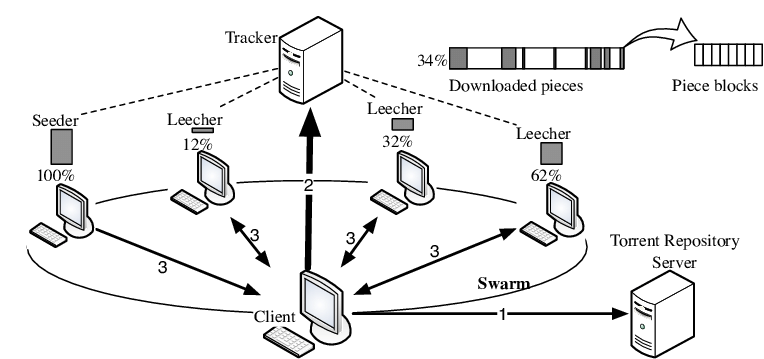
\includegraphics[scale=0.45]{img/bittorrent.png}
    \caption{Structure of the bitTorrent network}
\end{figure}
